%=========================================================================%
% Author: Pablo S�nchez                                                   %
% Paper: FOSD2010 (Case Study)                                            %
% Version: 1.0                                                            %
% Date   : 2010/05/07                                                     %
%=========================================================================%

This section presents the Smart Home Software Product Line case study~\footnote{\url{http://personales.unican.es/sanchezbp/CaseStrudies/SmartHome}}, which will be used through the paper to analyze if C\# partial classes are a suitable mechanism to achieve feature-oriented software development.
This case study was provided by Siemens in the context of the AMPLE project\footnote{\url{http://www.ample-project.net}}~\cite{Groher:2009,fuentes:2009,sanchez:2007,nebrera:2008}. We have selected it because it has demonstrated during the AMPLE project to be an excellent benchmark for Software Product Line Engineering; since it contains a wide range of variations of different kind and nature. Thus, it can be used to analyze if a new research contribution works properly in a wide range of potential situations.

A Smart Home software aims to improve comfort and security of the inhabitants of a house or a building, as well as to make a more efficient use of energy and resources. To achieve this goal, the software is in charge of controlling and coordinating a set of devices, such as doors, lights, heaters, windows and so forth.
Figure~\ref{fig:SH-FM} depicts a feature model for our Smart Home case study. It has been simplified for the sake of brevity. A complete version can be found in S{\'a}nchez et al~\cite{sanchez:2007}.

\begin{figure}
  \begin{center}
    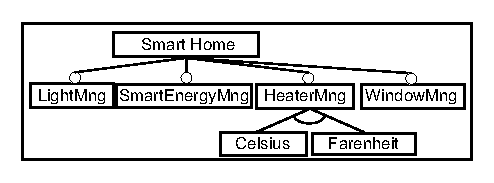
\includegraphics[width=.85\linewidth]{images/featureModel.eps} \\
    \caption{Smart Home feature model}
    \vspace{-15pt}
      \label{fig:SH-FM}
  \end{center}
\end{figure}

It specifies a Smart Home can optionally manage lights, windows and heaters. Moreover, there is a smart energy option which coordinates windows and heaters for save energy. For instance, before heating a room, if outside temperature is colder the software close the windows to avoid wasting energy. Obviously, this function required the heater and window function has been selected, which is specified by means of a required relationship.

Figure~\ref{fig:SH-DM} shows a UML model depicting a design supporting the variations specified for the previous feature model. Each coarse-grained feature, such as \imp{LightMng} is encapsulated in a UML package, as established by the feature-oriented design guidelines elaborated in the AMPLE project~\cite{sanchez:2007,nebrera:2008}. These packages are combined using UML merge relationships. UML merge relationships, roughly speaking, merge those elements of the same kind which match by name.
% Improve this
For instance, \imp{Gateway} classes will be merged to produce a combined version. Fine-grained variations are accommodated using other techniques, such as parametrization. So, variation in heaters measurement units is achieved by setting appropriately up an attribute in the \imp{HeaterCtrl} class.

%% Comment a little bit on the general arquitecture based on a gateway

\begin{figure}
  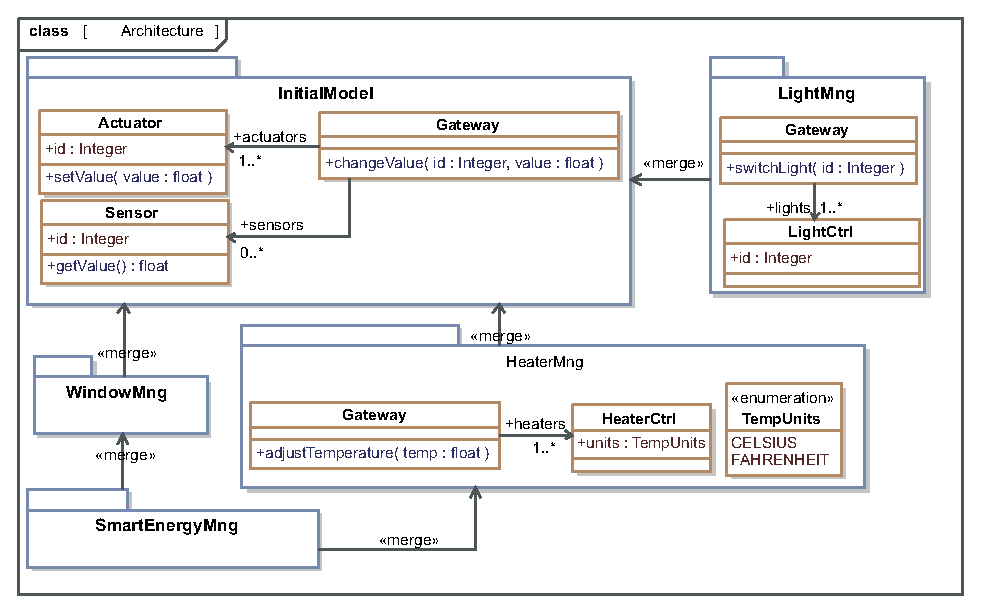
\includegraphics[width=\linewidth]{images/umlDesign.eps} \\
  \caption{Smart Home design}
  \label{fig:SH-DM}
\end{figure}

In the following sections, we will try to create an implementation of this feature-oriented design in C\# using partial classes. Strengthens and weaknesses of this technique will be identified.
